\begin{frame}{Considered Use Case}

  \begin{columns}
    \begin{column}{0.5\textwidth}
      \textbf{CSFL for collaborative IDS}
      \begin{itemize}
        \item One NIDS and one monitored network per organization.
        \item Objective: improve their local detection performance.
        \item Means:
        \begin{itemize}
          \item expert knowledge (\ie, datasets),
          \item computing resources (\ie, model training).
        \end{itemize}
      \end{itemize}
    \end{column}
    
    \begin{column}{0.5\textwidth}
      \begin{figure}
        \centering
        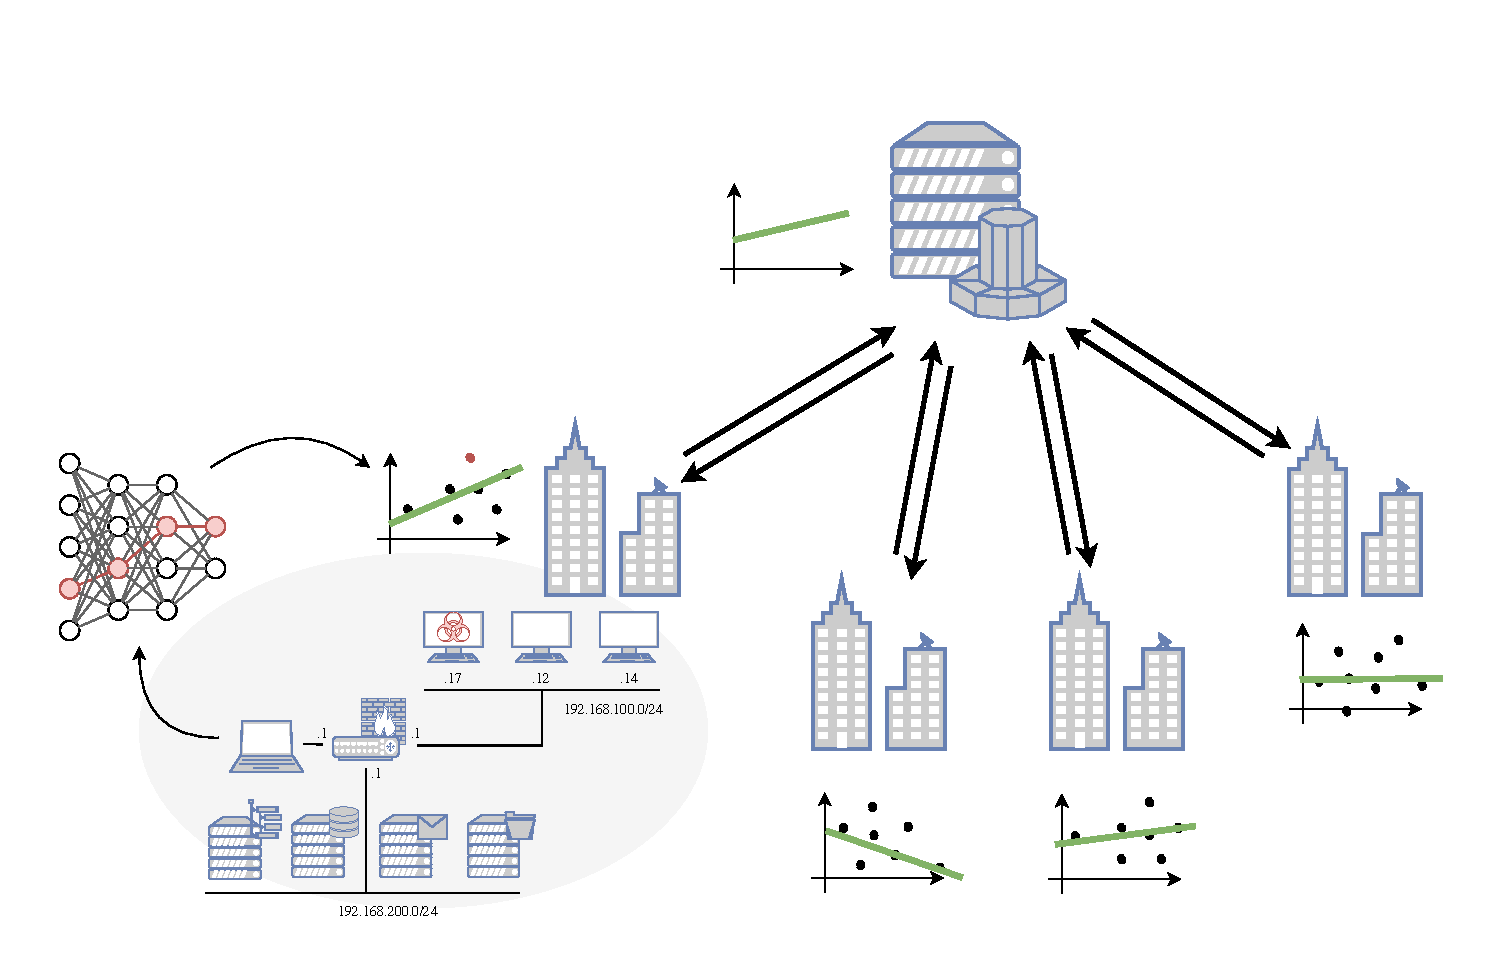
\includegraphics[width=1.1\linewidth,right]{figures/feditn/intro/cids.drawio.pdf}
      \end{figure}
    \end{column}
  \end{columns}
\end{frame}

\begin{frame}{Datasets}
\input{figures/feditn/backup/datasets-table.tex}
\end{frame}
  
% \begin{frame}
%   \begin{minted}[fontsize=\small,baselinestretch=1.0]{json}
% {
%   "specs": {
%     "source": {
%       "name": "Attackers",
%       "types": [
%         "host"
%       ],
%       "default": "hostileuser"
%     },
%     "files": [],
%     "parameters": {
%       "target": {
%         "name": "Target",
%         "types": [
%           "host.nics.ip",
%           "ip"
%         ],
%         "default": "webserver"
%       }
%     }
%   }
% }
%   \end{minted}
% \end{frame}